\section{Test}

\subsection{Step Respons Tilt}

For at lave en black box model af motoren, skal step responsen for omdrejningerne i forhold til spændingen over motorterminalerne findes. Det vil, med andre ord, sige at ændringen i motoromdrejningerne over tid skal måles ved en konstant spænding. Da motoren allerede er udstyret med en encoder, er det muligt at måle omdrejningshastigheden fra de to hall sensorer ved hjælp af en logic analyzer. Denne analyzer gør det muligt, at se hvor lang tid der går imellem flankerne på pulserne fra hall sensorerne, og på den måde udregne vinkelhastigheden derfra. 
Hver hall sensor giver 3 pulser på en omgang - det svarer til $\pi/3$ radianer fra en rising edge til en falling edge og omvendt. Logic analyzeren tilsluttes de to hall sensorer, og måler motorens respons i det øjeblik en konstant spænding på 12V sættes over motorterminalerne. Testen udføres 5 gange for at kunne sammenligne resultaterne. 

Når målingerne fra hall-sensorerne er regnet om til $rad/s$ og slået sammen til ét plot, produceres et plot der er meget støjet. Ud fra plottet på figur \ref{fig:Ubehandlet} kan man se at støjen er periodisk - det skyldes primært to faktorer: Hvis hall sensorerne ikke sidder præcist 90 grader forskudt, vil afstanden imellem flankerne på signalet heller ikke altid passe med $\pi/3$ radianer, som det er antaget i udregningen af vinkelhastigheden. Det vil resultere i hastigheder, der er enten for høje eller for lave i forhold til virkeligheden - denne fejl vil gentage sig periodisk fordi afvigelsen fra $\pi/3$ radianer vil være den samme altid. Den anden faktor, der har samme effekt på plottet, er polerne i rotoren - de vil heller aldrig være forskudt med helt den samme vinkel.

\begin{figure}[ht]
	\begin{center}
		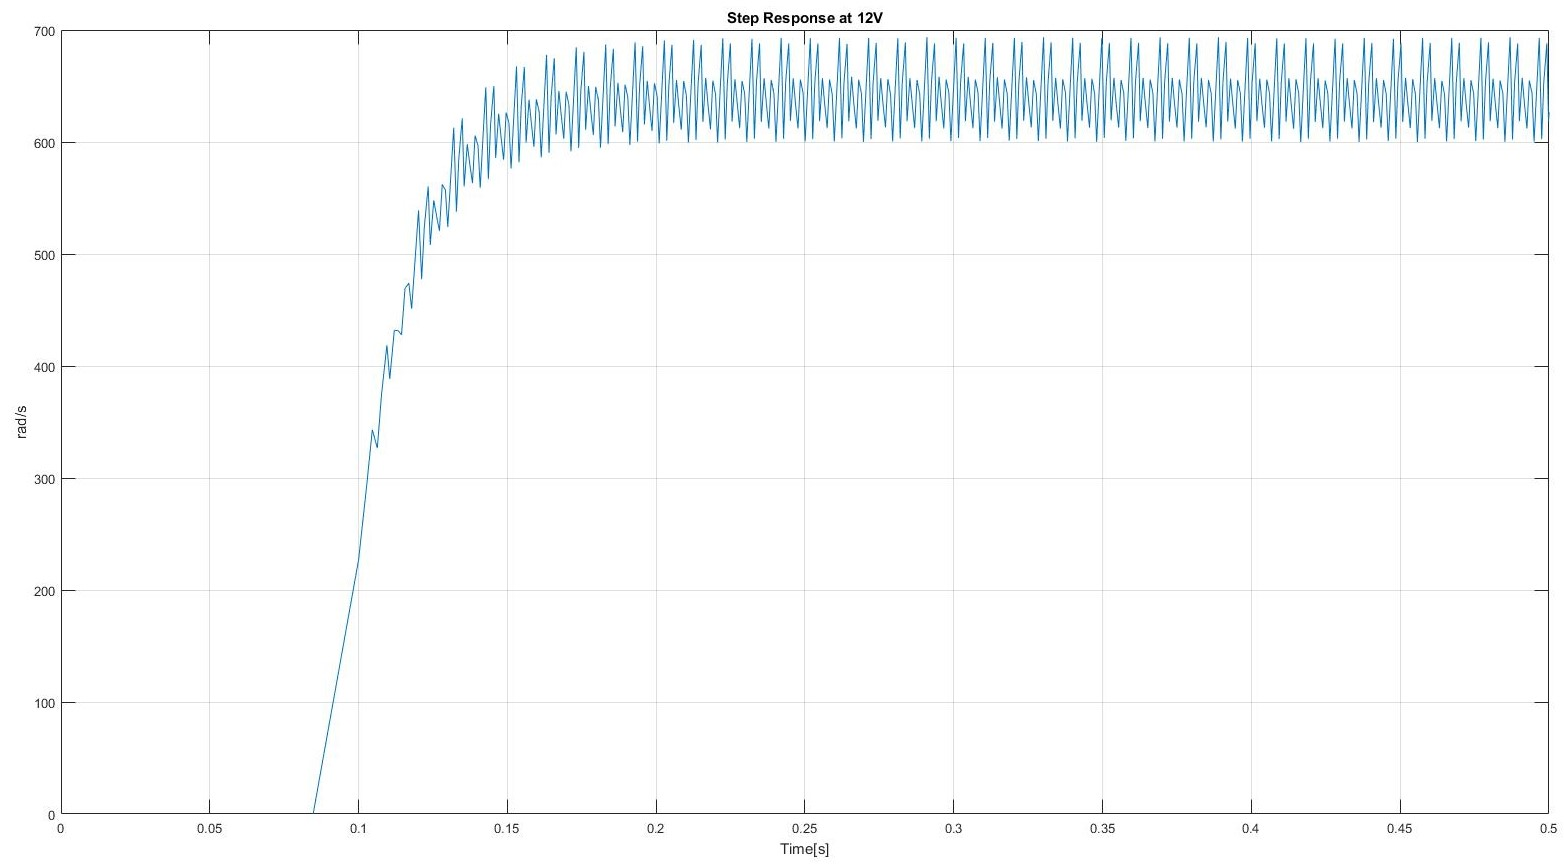
\includegraphics[scale=0.35]{Billeder/Untreated_Response.jpg}
	\end{center}
\caption{Den målte step respons i rad/s ved 12V konstant spænding. Omdrejningshastigheden er beregnet ud fra tiden imellem flankerne på hall sensor-signalerne. Der er interpoleret ned til 0 rad/s ud fra hældningen på de første to målinger.}
\label{fig:Ubehandlet}
\end{figure}

Hvis man nærstuderer figur \ref{fig:Ubehandlet}, kan man se at udsvingene gentager sig selv hver 12. sample. Det passer perfekt med at hver hall sensor har 6 halvperioder, hvor der bliver målt en tid, pr omgang. Det er med andre ord muligt at justere for fejlen ved at gange en faktor på alle samples, der tager højde for afvigelsen fra de $\pi/3$ radianer. I matlab kan man relativt simpelt finde de 12 faktorer, ved at undersøge hvor meget 12 konsekutive samples afviger fra gennemsnittet, så længe det bliver gjort i et område hvor responsen har nået steady state. Så er det bare et spørgsmål om at gange faktorerne på alle samples med det rette offset for at justere for fejlen. 

\begin{figure}[ht]
	\begin{center}
		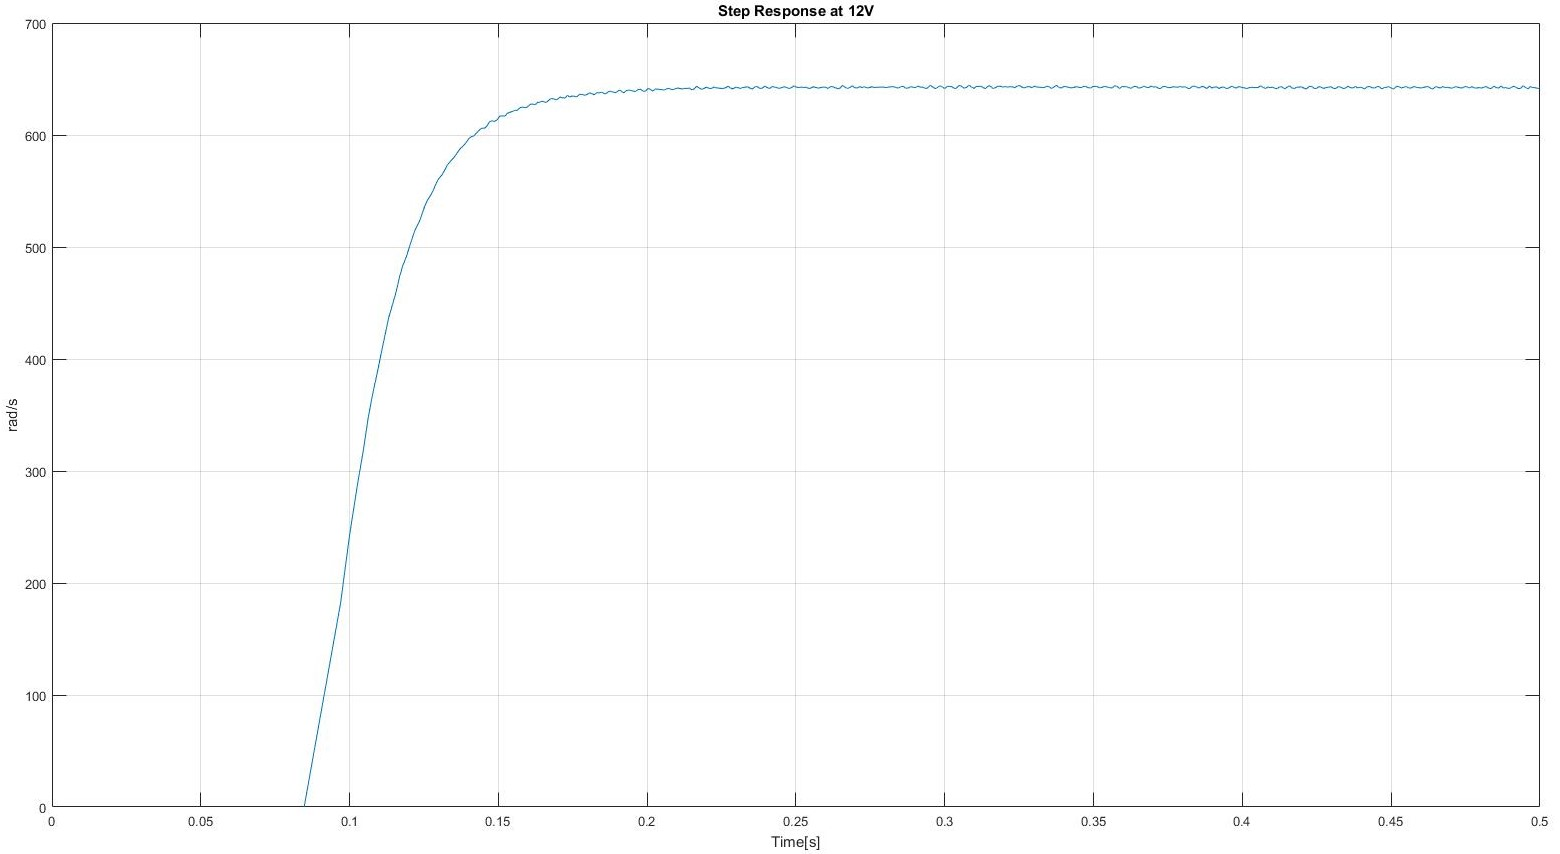
\includegraphics[scale=0.35]{Billeder/Treated_Response.jpg}
	\end{center}
\caption{Den målte step respons justeret for periodiske fejl.}
\label{fig:Behandlet}
\end{figure}

På det nye plot det noget lettere at aflæse tidskonstanten for systemet. Den eneste store usikkerhed der er tilbage er starttidspunktet for steppet, da det ikke indgår i målingerne fra logic analyzeren - det er en tilnærmet værdi ud fra hældningen af de første par samples ($\Delta\omega/\Delta t$). Plottene på figur \ref{fig:Ubehandlet} og \ref{fig:Behandlet} viser responsen for motoren uden belastning. Den aflæste tidskonstant på figur \ref{fig:Behandlet} er 27.3 ms.

Samme metode kan bruges til at måle step-responsen for motoren med belastning, så man kan få et billede af hvilken effekt den ekstra modstand har på systemet. På figur \ref{fig:Combined} kan man se responsen for motoren uden belastning, motoren kun med tilt-rammen, motoren med tilt-rammen og kamerabeslag og motoren med tilt-rammen, beslag og kamera monteret. Det er tydeligt at rammernes afbalancering har en stor indflydelse på responsen.

\begin{figure}[ht]
	\begin{center}
		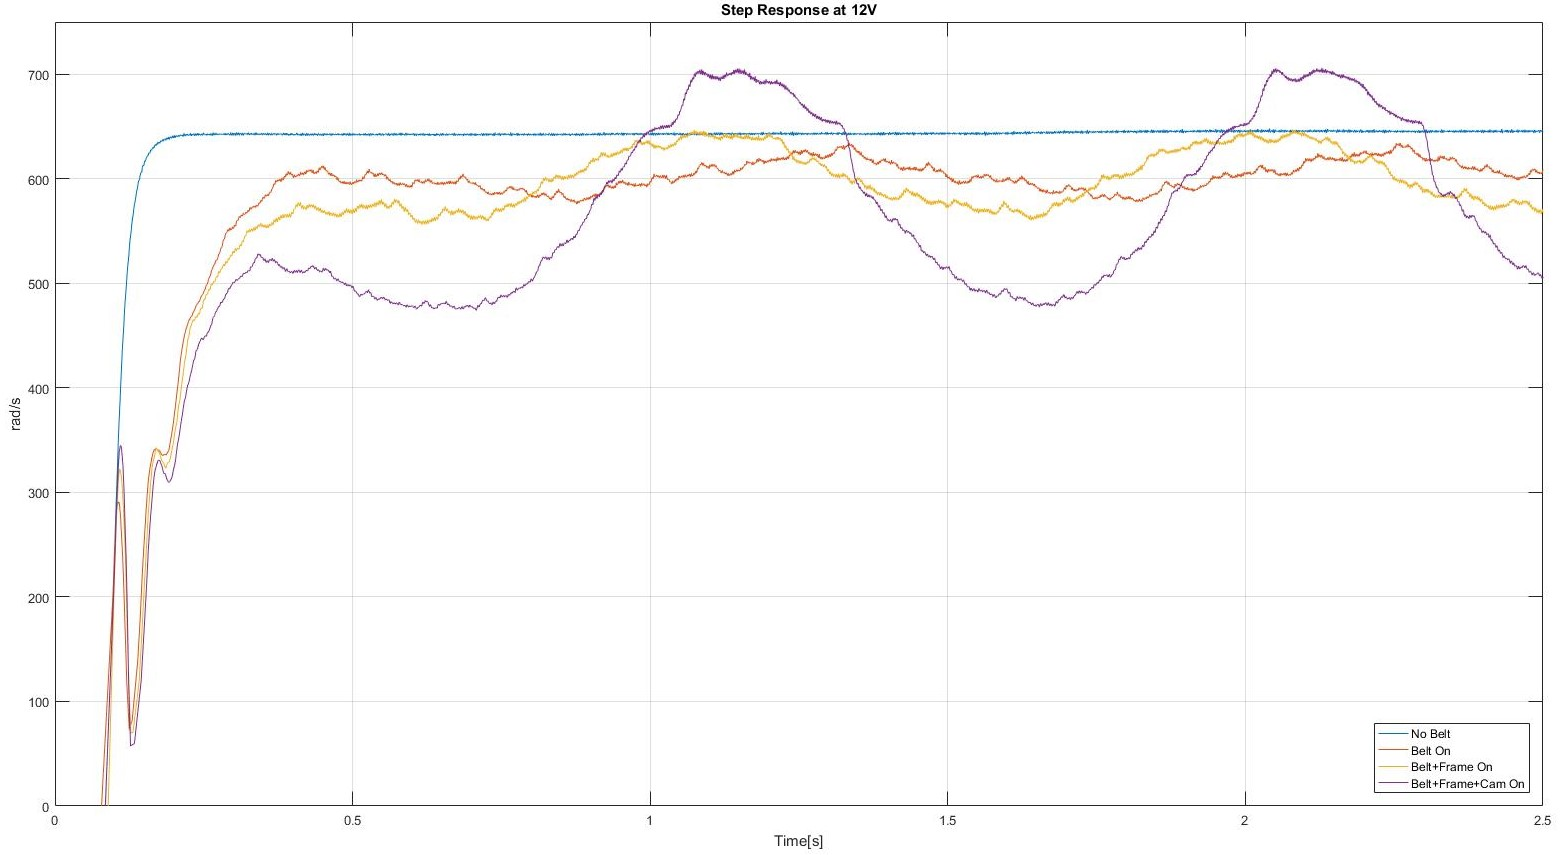
\includegraphics[scale=0.35]{Billeder/Response_Combined.jpg}
	\end{center}
	\caption{Step Respons for tilt-rammen med forskellig belastning.}
	\label{fig:Combined}
\end{figure}

Det kan også ses, at responsen for motoren, når den er forbundet med rammen, følger responsen for motoren uden belastning det første korte stykke tid, hvorefter hastigheden falder markant. En forklaring kunne være slør i forbindelsen mellem motoren og rammen - i den situation kan den fysiske modstand fra rammen først mærkes af motoren, når bælterne er blevet trukket helt i spænd. En anden ting der også er tydelig er, at selv når der ikke er monteret ekstra udstyr på rammen, så er der stadig en ubalance i rammen, der får hastigheden til at være ujævn over en hel omgang.

Det er stadigvæk muligt at approksimere systemet som et 1.-ordenssystem, men modellen vil udelukkende beskrive, hvor hurtigt systemet reagerer på inputs og ikke så meget om den præcise opførsel. Det vil dog være en rigtig god ide, at få afbalanceret rammerne så godt som muligt og gøre modstanden nogenlunde konstant over en hel omgang, for at modellen kan afspejle virkeligheden så godt som muligt. Med rammen forbundet med motoren er tidskonstanten omkring 125 ms.

\subsection{Step Respons Pan}



\subsection{Omdrejningshastighed vs Duty Cycle}

En af antagelserne der bliver gjort i modellen af systemet, er at der findes en nogenlunde lineær sammenhæng imellem duty cycle og omdrejningshastigheden. For at påvise denne sammenhæng kan man plotte hastigheden, når motoren har nået steady state, ved forskellige duty cycles. 

XXXX Do your stuffs here, Jonas/William

Hvis man plotter step responsen ved forskellige duty cycles (figur \ref{fig:RPM_DC}), kan det også påvises at tidskonstanten forbliver nogenlunde konstant. 

\begin{figure}[ht]
	\begin{center}
		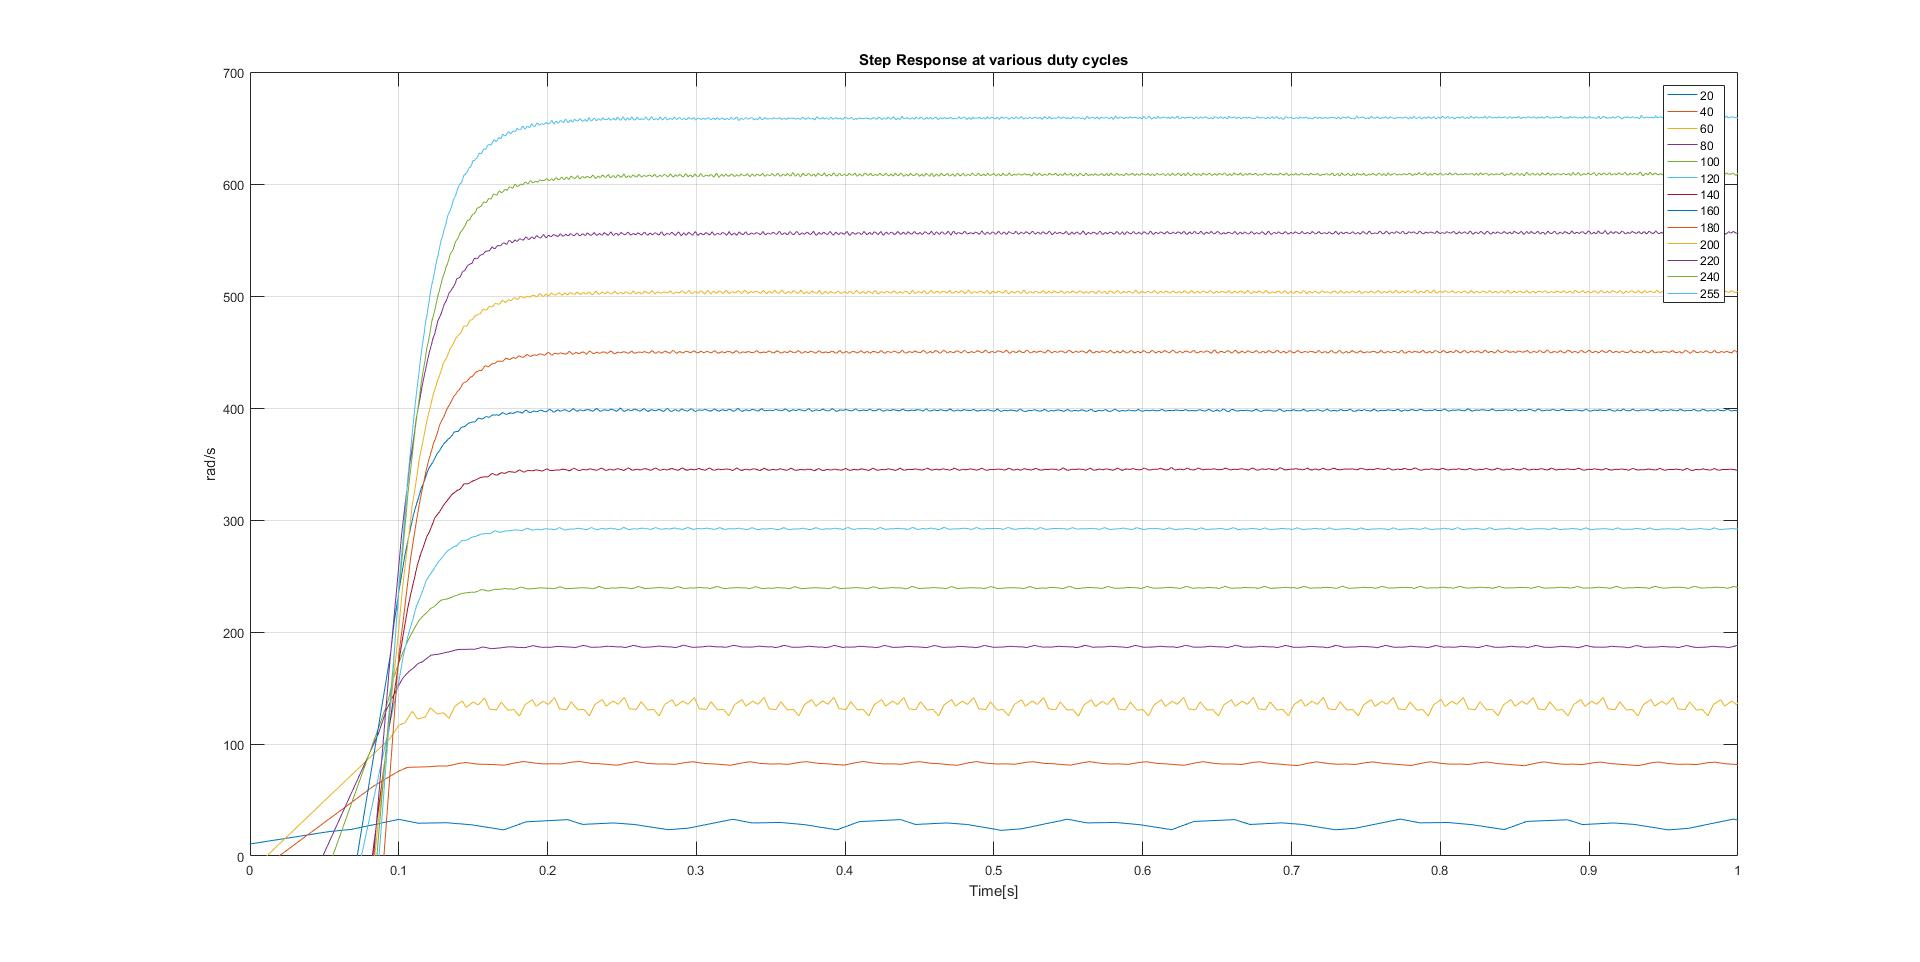
\includegraphics[scale=0.35]{Billeder/RPM_vs_DC.jpg}
	\end{center}
	\caption{Step Respons for tilt-rammen ved forskellige duty cycles}
	\label{fig:RPM_DC}
\end{figure}